\documentclass[10pt, twoside, a4paper]{article}
\usepackage[italian]{babel}
\usepackage[utf8]{inputenc}
\usepackage{amsmath}
\usepackage{amsfonts}
\usepackage{fullpage}
\usepackage[pdftex]{graphicx}
%\usepackage{booktabs} %ho provato a toglierlo per far meglio la tabella
\usepackage{wrapfig}
\usepackage{multirow}
\usepackage[rightcaption]{sidecap}
\usepackage{subcaption}
\usepackage{siunitx}
\usepackage[font=small]{caption}
\usepackage[bookmarks, hidelinks]{hyperref}
\usepackage{float}
%nuovi pacchetti
\usepackage{fontenc}
\usepackage{fancyhdr}
\usepackage{amssymb}
\usepackage{enumitem}
\usepackage[a4paper, top=1.4cm, bottom=1.4cm, left=1.5cm, right=1.5cm] {geometry}
\usepackage{multicol}
% per far meglio la tabella
\usepackage{array}

\begin{document}

\begin{center}

     	{\huge Amplificatori operazionali}

     	\vspace{0.2cm}
	\vspace{0.3cm}

      	{\large Alessandro Martinelli, Davide Bazzanella} \\
%     	{Bazzanella.Davide@gmail.com} \\
		{ Gruppo B10} \\
	
	\vspace{0.1cm}
      	{ 27 maggio 2014 }

\end{center}

Mediante l'oscilloscopio, verificare la funzione di trasferimento per filtri passa basso, passa banda e reiezione di banda.\begin{wrapfigure}[6]{r}[0pt]{130mm}
	\centering
    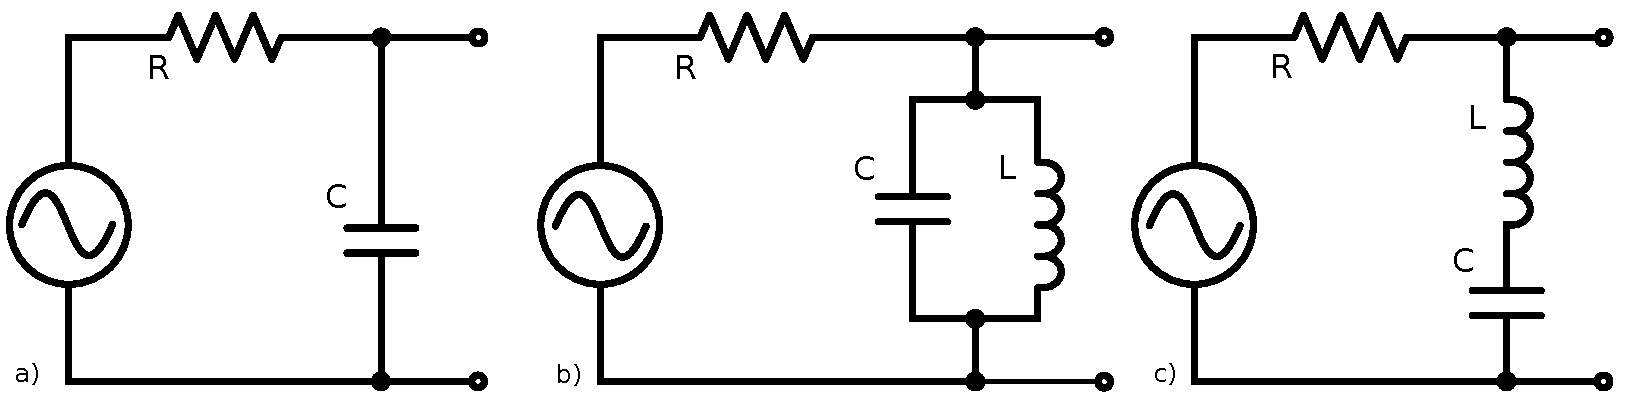
\includegraphics[width=0.7\textwidth]{circuiti.pdf}
    \caption{Schema dei circuiti utilizzati: a) filtro passa basso; b) filtro passa banda; c) filtro a reiezione di banda}
    \label{fig:circuito}
\end{wrapfigure}

\section{Strumenti}

$\bullet \quad$Oscilloscopio \\
$\bullet \quad$Cablaggio\\
$\bullet \quad$Breadboard (basetta sperimentale)\\
$\bullet \quad$Generatore di forme d'onda\\
$\bullet \quad$Multimetro digitale\\
$\bullet \quad$Decadi di resistenze,\\
\hspace{20pt} capacitori e induttanze\\

\section{Sorgente di corrente costante}
Prima di montare il circuito riportato in Fig.(), abbiamo dimensionato le resistenze $R_1$ e $R_2$ del partitore in modo da avere una sorgente di corrente costante $I_L=1\si{\milli\ampere}$. Avendo scelto come $R_E=(997.3 \pm 0.2)\si{\ohm}$ e utilizzando la relazione $I_L+I_B=I_E \Rightarrow I_L \approx I_E$ \footnote{Nei transistor la corrente di base è circa 100 volte inferiore rispetto a quella di collettore ed emettitore.} possiamo facilmente calcolare la tensione di base necessaria per fornire una $I_L=1\si{\milli\ampere}$: $V_B=I_L \cdot R_E + 0.6V$. Il secondo termine deriva dal fatto che tra base ed emettitore, essendo una giunzione p-n, vi è una caduta di tensione pari a $0.6V$.

Risulta immediato impostare dunque l'equazione che permette di calcolare i valori delle resistenze nel partitore:

\begin{equation}
\frac{R_2}{R_1+R_2} V_{CC}=I_L \cdot R_E + 0.6V
\label{partitore}
\end{equation}

Evidentemente i valori delle resistenze non sono univocamente determinati da Eq.(\ref{partitore}). Sarà dunque nostro compito scegliere una delle due in modo che non venga dissipata troppa potenza sul partitore e contemporaneamente scorra abbastanza corrente attraverso la base del transistor. \`E stata scelta $R_1=99.06 \pm 0.1 \si{\kilo\ohm}$, valore che ci sembrava adeguato per soddisfare le due caratteristiche sopra citate. 

Da Eq.(\ref{partitore}) risulta $R_2 = 18.6\si{\kilo\ohm} $. Il valore effettivamente utilizzato nel circuito è stato $R_2 = (18.01 \pm 0.2 )\si{\kilo\ohm} $. Tale lieve discrepanza non influenzerà certamente la bontà dell'esperimento. Infatti anche il transistor, in base alla temperatura dell'ambiente, avrà delle variazioni considerevoli delle caratteristiche intrinseche. Ci aspettiamo dunque che il valore di corrente che successivamente andremo a misurare non avrà un valore esatto di $1\si{\milli\ampere}$. 
Riportiamo ora un grafico di $I_L$ in funzione del carico.

$$Grafico$$

Ricordiamo anzitutto che avendo avuto una $I_L<1\si{\milli\ampere}$ per qualsiasi carico, abbiamo utilizzato il multimetro in modalità amperometro con un fondo-scala di $1\si{\milli\ampere}$ senza mai cambiarlo (così facendo abbiamo evitato di dover correggere i dati per le diverse resistenze interna dello strumento stesso).

Come si vede graficamente, per valore di $R_L<stocazzo$, il valore di corrente di collettore è pressoché costante. Per valori di $R_L>stocazzo$ la corrente decresce. Ciò è dovuto al fatto che, se la differenza di tensione collettore-emettitore è inferiore a $0.2V$, il transistor entra in saturazione e a quel punto la corrente di  collettore non è più determinata dalla corrente di base ma dal carico $R_L$. Risulta immediato verificare che  per un valore di carico superiore a $stocazzo$ i dati obbediscono ad una legge lineare. 

**dati del fit e spiegare se è possibile stimare Vce dai dati**   

\section{Amplificatore ad emettitore comune}

Riportiamo in Fig.() lo schema del circuito utilizzato per questa seconda parte dell'esperienza. Anche in questo caso abbiamo dovuto dimensionare le resistenze del partitore e inoltre anche la capacità $C_1$. Avendo scelto come $R_E=(498.4\pm0.1)\si{\ohm}$ e volendo una corrente di quiescenza di $\approx 1\si{\milli\ampere}$ abbiamo stimato $V_B=1.1V$. Possiamo ora, attraverso Eq.(\ref{partitore}), calcolare i valori di $R_1$ e $R_2$. Avendo anche in questo caso scelto $R_1=(100.03\pm0.2)\si{\kilo\ohm}$ abbiamo utilizzato una $R_2=(12.16\pm0.01)\si{\kilo\ohm}$. Come segnale in ingresso è stata usata una forma d'onda sinusoidale a frequenza di $1\si{\kilo\hertz}$. Per la struttura del circuito risulta semplice impostare il calcolo di $C_1$. Infatti il condensatore è caricato dal parallelo delle resistenze del partitore. Inoltre, esso fa parte di una sorta di filtro passa alto. Basterà dunque utilizzare dei valori di capacità adeguati in modo da avere una frequenza di taglio minore di $1\si{\kilo\hertz}$. Riportiamo ora l'equazione utilizzata per il calcolo di $C_1$

\begin{equation}
C_1>>\frac{1}{2 \pi \cdot R_1 // R_2}
\end{equation}

Inserendo i nostri valori, otteniamo $C_1>>15\si{\nano\farad}$. E' stato dunque scelto di usare un uno dei primi condensatori trovati sul tavolo con capacità $C_1=(0.982\pm0.005)\si{\micro\farad}$. 

Per la nostra esperienza era richiesto un guadagno in tensione pari a $G=-10$. Ricordando che $G\doteqdot \frac{e^{i\pi}R_C}{R_E}$ è stato immediato pickare una $R_C=(4.969\pm0.001)\si{\kilo\ohm}$. 

Stimati tutti i valori delle componenti circuitali, abbiamo montato il circuito vero e riportando a schermo dell'oscilloscopio sia segnale in ingresso che in uscita. Nel seguente grafico sono riportati i dati dell'oscilloscopio.

$$Grafico$$

Come vediamo immediatamente, il segnale in uscita è sfasato di $\pi$. Proprio per questo motivo nella formula del guadagno compare quel $e^{i\pi}$. Dai dati sperimentali è stato possibile stimare il valore di guadagno effettivo, utilizzando la tensione picco-picco:

$$G_{exp}=e^{i 0.9972 \pi} suca$$

\section{Caratteristica di uscita}

In questa ultima parte dell'esperienza abbiamo cercato di analizzare la caratteristica di uscita del transistor. Per fare ciò abbiamo montato il circuito in Fig.(). Alimentandolo con un'onda sinusoidale di frequenza $1\si{\kilo\hertz}$, con tensione picco-picco di $10V$ e offset di $+5V \, DC$ e impostando l'oscilloscopio in configurazione XY, possiamo ottenere la caratteristica di uscita per diverse correnti di base (impostate cambiando la $V_B$). 
\newpage
\noindent \begin{minipage}{\linewidth}
Inoltre notiamo che la fase non è quella tipica del filtro notch già studiato nella precedente esperienza. Questo è dovuto al fatto che noi abbiamo considerato la differenza di fase tra i due segnali ai capi del ponte di Wien, non tra segnale in input e differenza dei due segnali in output. Tale relazione risulta infatti essere:

\begin{equation}
\vartheta_{out|in}=arctan\left[\frac{2 C R \omega \left(C^2 R^2 \omega^2-1\right)}{C^4 R^4 \omega^4+C^2 R^2 \omega^2+1}\right]
\label{teo}
\end{equation}

Poichè non è stata rilevata la differenza di fase direttamente durante l'esperienza, essa è stata calcolata dai dati sperimentali imponendo la condizione, valida per ogni $t$:

\begin{equation}
V_{out}sin(\omega t + \vartheta)=V(CH1)sin(\omega t + \varphi)-V(CH2)sin(\omega t)
\end{equation}

Scegliendo come tempo $t=0$, e applicando un arcoseno, otteniamo subito lo sfasamento del segnale in uscita rispetto a quello in entrata.

\begin{equation}
\vartheta=asin\left(\frac{V(CH1)}{V_{out}}sin(\varphi)\right)
\label{dati}
\end{equation}


Riportiamo in Fig \ref{fig:pahser} la legge teorica (\ref{teo}) e dati sperimentali rielaborati attraverso (\ref{dati}). Nonostante la propagazione degli errori, nel grafico non sono ancora distinguibili le barre d'errore.
\end{minipage}

% questa dovrebbe essere la fase GIUSTA (da mettere a parte) y=180/pi*np.arctan((2*C*R*w*(-1 + (C*R*w)**2))/(1 + (C*R*w)**2 + (C*R*w)**4))

\section{Conclusioni}
\noindent \begin{minipage}{\linewidth}
Attraverso il ponte di Wien siamo riusciti ad ottenere una misura precisa del valore di un capacitore incognito. Un valore compatibile con quello misurato dal multimetro e dichiarato dal costruttore è ottenibile sia dalle equazioni di bilanciamento che dalla loro combinazione. Notiamo dai dati riportati in tabella che quest'ultimo procedimento è quello che permette una stima affetta da minor errore. 
Abbiamo verificato il funzionamento del ponte di Wien come filtro notch. Esso, come già detto, non risulta efficace come un filtro notch costruito utilizzando capacitore in serie ad un'induttanza. Inoltre, per le scelte da noi fatte di resistenze e capacità, l'intensità picco-picco del segnale in output non potrà mai essere superiore a $\frac{V_{in}}{2}$.
\end{minipage}

\begin{figure}[H]%[30]
	\centering
	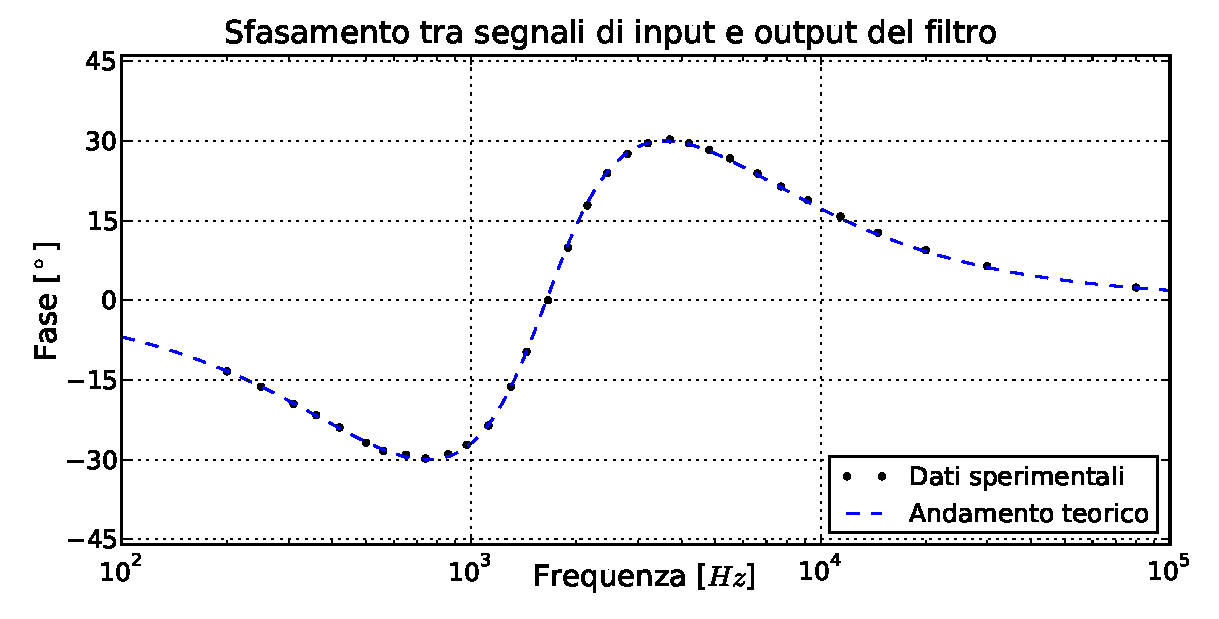
\includegraphics[width=150mm]{i_peli.pdf}
		\caption{Nel grafico sono riportati i valori di differenza di fase tra il segnale in input al circuito e il segnale in output. Ricordiamo che i dati sperimentali sono stati rielaborati usando la formula (\ref{dati}).}
	\label{fig:pahser}
\end{figure}
\end{document}